%\documentclass[12pt,a4paper]{article}
%\usepackage[latin1]{inputenc}
%\usepackage{amsmath}
%\usepackage{amsfonts}
%\usepackage{amssymb}
%\usepackage{graphicx}
%\author{Iason Filippopoulos \and Francky Catthoor \and Per Gunnar Kjeldsberg}
%\title{Technology scaling impact on the interconnect of clustered scratchpad memory architectures}

%\begin{document}
%\maketitle


\chapter{Technology scaling impact on the interconnection of clustered scratchpad memory architectures}

\begin{center}
Iason Filippopoulos, Francky Catthoor, Per Gunnar Kjeldsberg
\\
To be submitted
\\
2015
\end{center}
\afterpage{\null\newpage}
\newpage

\vspace*{\fill}
\section*{\hspace*{\fill} Abstract \hspace*{\fill}}
Power consumption is the key limitation in modern embedded devices.
The memory architecture contributes significantly on the overall power consumption of the system.
Among other proposed techniques, one effective system design approach to reduce the memory power needs is the design of a dynamically reconfigurable clustered memory architecture.
The operationally independent memory banks provide an energy efficient platform, but comes with an interconnection overhead due to the connections between the memory banks. 
Thus, there is a trade-off between the energy gains by increasing the number of memory banks and the increase on the interconnection overhead.
This work explores the future development of the interconnection overhead, as the interconnection cost is expected to increase while the process technology shrinks to 5nm.
The current study employs both CAD tools with simulation results using the current technology and projections provided by institutions.
We use predictive technology models and the quantitative data are supported partly by information
from ITRS and IMEC's interconnect technologists.
A model is developed that provide rough estimation about the interconnection cost overhead for clustered memory architectures consisting of two to five memory banks and a range of technologies from 40nm to 5nm.  
\vspace*{\fill}
\afterpage{\null\newpage}
\newpage

\section{Introduction}

Embedded systems normally rely on battery and this fact reduces their usability.
The power consumption can be divided between the processing elements and the memory subsystem.
One efficient way to reduce the power consumed on the memory, when executing an application with dynamic memory needs, is to design a clustered memory architecture.
A case study about the efficiency and the potential gains of this approach is presented in \cite{filippopoulos2013exploration}.
In Fig.\ref{fig:platformE} the two different approaches are presented.
The first has a large static memory and the second five smaller memory banks, while designer can choose other alternatives in between.
The different memory banks can operate independently and  adjust to the application requirements.
When the memory requirements of the application are small, unused memory banks can be switched off and the energy consumption is reduced, while the application still runs successfully on the system. 

\begin{figure}
 \centering
 \includegraphics[width = \textwidth]{E/platform.pdf}
  \caption{The alternative clustered memory architectures ranging from one to five memory banks}
 \label{fig:platformE}
 \end{figure}
 
 The main drawback of the clustered memory architecture approach is the need for extra interconnection circuit.
 Unfortunately, it is expected that the interconnection networks will take up an increasingly significant portion of system power in the system. 
Thus, there is a need to obtain a detailed memory and interconnect energy model including the scaling impact. 
That will allow to accurately incorporate the interconnection cost overhead in our studies. 
That will allow to decide whether and when the power gains justify the use of a clustered memory architecture instead of a monolithic one. 
But it especially also allows to identify the best trade-off working points between using more
or less memory banks within the clustered approach. 
Without this, an overly optimistic distribution across too many banks would seem to provide the
best energy for a given application requirement.
  The scope of this work is explores the future development of the interconnection overhead and develop a model that can provide rough estimation about that overhead.
  System designers could use such a model to decide about the preferred memory architecture and the number of banks given the nature of the executed application and the target technology.
  The model is based on the current technology and the projections about the future technology.
  The current technology is available on several CAD tools.
  The synthesis and the simulation of memory architectures similar to the one in Fig.\ref{fig:platformE} provide useful results.
  The study of the future technology is based on the reports released by the International Technology Roadmap for Semiconductors (ITRS) \cite{itrs}.
 The goal of the developed model is to provide rough estimation about the interconnection cost overhead for clustered memory architectures consisting of two to five memory banks and a range of technologies from 40nm to 5nm.  
 
 The paper is organized as follows. The ...

\section{Related Work}

A comprehensive view of a class of interconnect architectures is presented in \cite{kumar2005interconnections}. 
The authors examine the area, power, performance, and design issues for the on-chip interconnects.
A few more on current papers... \ldots

Successful examples of clustered memory arch ... \ldots

Overview of the ITRS based paper \ldots

\section{Current technology}
\label{Current}

\subsection{Generic Work-flow}

The current technology is studied as a first step towards the development of an interconnection cost model. 
CAD tools allow the design of the described clustered memory architectures.
The synthesis and the simulation provide reliable data for the area and the power consumption of the different parts of the memory architecture.
The goal is to synthesize a clustered memory architecture and extract power data for the memory banks and the interconnection logic separately.
The work-flow is divided in several sub-steps:

\begin{itemize}
	\item A number of memory banks is chosen from a library, which contains several SotA designs.
	\item An RTL description for connecting the memory banks into a full memory architecture design is written.
	\item A simulation is performed to verify the correct functionality of the memory architecture.
	\item A target technology is chosen and the logic synthesis of the memory architecture is performed.
	\item The floor-planning and the placing \& routing of the memory design is performed.
	\item The dynamic timing and the power simulation are performed and the results are provided.
\end{itemize}

Regarding the first step, the memory models are presented in \cite{filippopoulos2013exploration}.
The memory models include state-of-the-art standard cell-based memories (SCMEM) \cite{Mei11}, which are designed to be power efficient. 
The energy numbers for the SCMEM are also derived from synthesis and simulation results.
The presented work-flow is the typical procedure followed by an industry designer except the usage of SCMEM instead of other commercially available memory macros.
SCMEM are preferred for their characteristics and especially their energy and area efficiency for reasonably small storage capacities, as argued in \cite{Mei10}. 
Thus, the choice of using SCMEM is mostly related to the heavily distributed memory organization, which we target. 
The sizes of the memory banks in the target memory organization are too small to motivate a solution based on macro memory blocks, mainly because macro memories are dominated by the periphery.
Another factor for this decision is the fact that a rectangular cell array is not necessarily the optimal solution in terms of energy consumption.
The usage of the custom memories provide the freedom to explore different memory organizations by combining banks of different sizes and structures.  

For the second step, the RTL description connects the memories using MUX, signals and other components into a functional clustered memory architecture. 
On the third step, the simulation and the verification performs a flash-write followed by a read on the whole memory architecture. 
The target technology depends on the available libraries.
In this work, the TSMC library on 45nm is used.
The place and route can be either performed automatically through the CAD tool or manually by the designer.

The final step, includes the extraction of  parasitic, the static timing analysis and the annotation of the timing to the netlist.
Afterwords, power simulations on the synthesized design are carried out using Synopsys PrimeTime, in order to obtain energy numbers.

\subsection{Example design: synthesis and simulation}

A group of clustered memory architectures is designed and synthesized following the presented work-flow.
The simulation provides results for the current technology and the contribution of the interconnection to the overall energy consumption.
The study includes clustered memories with an increasing number of memory banks, beginning with only one memory bank and continue up to five memory banks.
There are two main reason for exploring architectures up to five memory banks.
Firstly, the energy gains achieved by increasing the number of memory banks in the memory architecture are nearly saturated even for five banks.
In \cite{filippopoulos2013exploration} a group of different applications were studied with regard to their energy consumption on a clustered memory architecture consisting of up to five memory banks.
The results shows that depending on the application, the energy gains started to saturate after adding a third or a fourth bank and become far smaller when adding a fifth bank.
Thus, for most applications a memory architecture with five memory banks already provides more than necessary reconfiguration options.  
Secondly, the overhead increases exponentially with the number of memory banks, due to the increased complexity of the memory architecture. 
The significant increase in the overhead is indicated by the synthesis results, especially while comparing the overhead between four and five memory banks.
Therefore, a memory architecture with six banks is not a potentially efficiency options due to the high overhead and the very low energy gain.

The breakdown of energy consumption is split into two parts of the memory.
The first part is the energy consumption inside each memory bank, which includes the memory cells, the necessary logic to connect the cells and the addressing circuit.
The second part is the interconnection cost between the different memory banks, which includes the necessary logic to locate and transfer the data outside of the banks. 
In other words, the interconnection outside the memory banks is given separately. 
The interconnection between the different memory cells inside one bank is included on the energy of the memory bank.

The energy breakdown between the first part of the memory banks and the second part of the interconnection (part2) is presented in Fig.\ref{fig:energyE}.
The energy cost of the interconnection logic is small compared to the energy cost for the write and read operations on the memory banks.
Tab.\ref{tab:overhead} contains the exact percentages of the energy overhead on the interconnection. 

\begin{figure}
 \centering
 \includegraphics[width = \textwidth]{E/energy.pdf}
  \caption{Energy breakdown between the memory banks and the interconnection}
 \label{fig:energyE}
 \end{figure}
 
 \begin{figure}
 \centering
 \includegraphics[width = \textwidth]{E/area.pdf}
  \caption{Area breakdown between the memory banks and the interconnection}
 \label{fig:areaE}
 \end{figure}
 
 \begin{table}[t!]
\caption{Percentage of energy overhead on interconnection}
\label{tab:overhead}
\centering
\begin{tabular}{|c|c|c|c|c|c|}
\hline 
Banks & 1 & 2 & 3 & 4 & 5 \\
\hline 
Overhead(\%) & 0	&	1.2627 & 1.3687 & 1.7683 & 3.0067 \\ 
 \hline 
 \end{tabular} 
\end{table} 
 
The changes in the area of the design is presented in Fig.\ref{fig:areaE}.
The area used for the placement of the memory banks is separated from the area occupied by the interconnection.
  
In addition, the synthesis and simulation of the memory designs provide useful information about the dimensions of the memory banks, the length and the capacitance of the wires.
Several interesting observations are possible based on the study of the current technology.
The energy overhead on the interconnection of the banks grows when there are more memory banks connected, as expected.
However, the overhead is just over 3\% even for a clustered memory with five banks. 
The area overhead is significantly higher and grows exponentially for an increasing number of memory banks.  
The maximum area overhead is less than 10\%.
This is explained by the need for extra wiring to connect the different memory banks.

\section{Technology Scaling}

The technology scaling projections are based on the reports released by the International Technology Roadmap for Semiconductors (ITRS) \cite{itrs}.
The clustered memory architecture can be divided into two parts, i.e. the memory banks and the interconnection.

\subsection{Memory Banks}

\begin{figure}
 \centering
 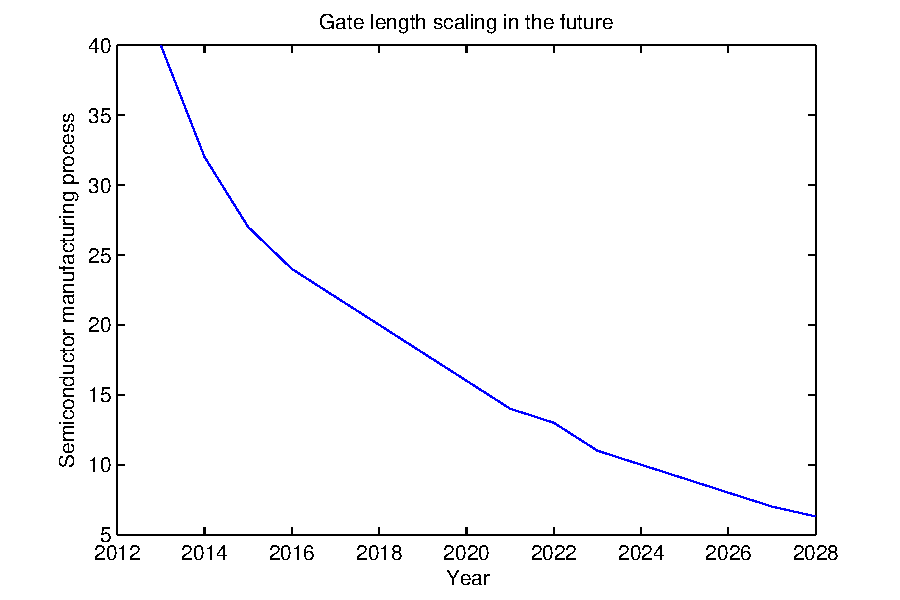
\includegraphics[width = \textwidth]{E/gate.pdf}
  \caption{Impact of technology scaling into gate length}
 \label{fig:gateE}
 \end{figure}
 
  \begin{figure}
 \centering
 \includegraphics[width = \textwidth]{E/cellpower.pdf}
  \caption{Normalized dynamic power and technology scaling}
 \label{fig:powerE}
 \end{figure}
 
The memory banks consist of the memory cells, which are built using gates.
Thus, the predictions about the future behavior of the memory banks is based on the ITRS reports for logic.
In the following years, the gate of the length is expected to be reduced as shown in \ref{fig:gateE}.
The values are approaching 5nm around 2028, which is potentially the limit using the current manufacturing process.

The reduction on the gate length leads to a reduction of the memory cell and naturally smaller memory banks.
The smaller memory banks affect the area of the design and the power consumption.
The projections provided by ITRS regarding the power are presented in \ref{fig:powerE}. 
There is a significant reduction on the power consumption in the short term and slighter reduction at the end of the projections.

\subsection{Interconnection}

The interconnection cost is based on the projections about wiring, which differentiate compared to the projections regarding the logic gates.
The current study is restricted to the reports about the lower and intermediate metal layers, because these are the ones that are relevant for the interconnection on our memory organizations.
The reports about the global interconnection scaling is not our focus, as it is used for the power and clock routing and among computing clusters on a large platform SoC.
However, the change on the size of the memory banks affects the length of the needed wires.
The most important parameters for the current study is the capacitance and the power of the interconnection.
Based on the data provided by ITRS, the curves for the two parameters are presented in \ref{fig:intpowerE}.
The capacitance is expected to be reduced in the following year.
However, the rate of reduction is lower compared to the expected reduction for the memory banks.
The power values are per length unit and there are expected to raise due to the several challenges that the interconnection technology will face in the future.

 \begin{figure}
 \centering
 \includegraphics[width = \textwidth]{E/intpower.pdf}
  \caption{Impact of technology scaling into the capacitance and the power of the interconnection part}
 \label{fig:intpowerE}
 \end{figure}

The significant parameter in this work is the capacitance and not the resistance.
Resistance is also generally studied in the interconnection, because it has an important impact especially for
delay. 
The current work focus on energy rather than delay and this is a rational choice for embedded systems.
In general, the clock speeds are relatively low for a typical embedded systems in contrast to high performance computing.
In our target domain, a system architecture includes several processing cores that can be of different types to fulfill different application requirements.
When higher performance is needed in an embedded system, it is usually achieved by adding another processing core or a special hardware unit rather than having an extremely high clock speed.
Thus, it is expected that the critical path delay is not the main worry for a system designer.
If the aim is high-performance designs, the current work has to be extend in the future.
A different approach where delay-energy trade-offs are incorporated
from the start should be developed in such a case.

\section{Model Construction and Projection Results}

 \begin{figure}
 \centering
 \includegraphics[width = \textwidth]{E/overhead.pdf}
  \caption{Projections of the interconnection cost power overhead for different numbers of memory banks}
 \label{fig:overheadE}
 \end{figure}

 The scope is to develop a model that can provide a rough estimation on the power overhead for the interconnection on clustered memory architectures.
 The model is based on the synthesis results of the currently feasible designs and study of the projections provided by ITRS.
 The input for the model is the process technology and the number of memory banks.
 The power consumption on the memory banks is calculated using Fig.\ref{fig:powerE}.
  The prediction of the power consumption on the interconnection logic is more complex.
 Based on the technology and the number of memory banks, the length of the wires is calculated and sequentially the capacitance.
 Normally the power consumption is given as  $Power = \dfrac{1}{2} \times f \times C \times V^{2} $, where  f is the operating frequency, C the capacitance and V the supply voltage.
 However, the simulation results and the projections provided by ITRS suggest that a more complex model of computation is needed.
 
 The model of computation for the interconnection power cost overhead for a given target technology $ t $ and a number of $ n $ banks of 1KB  is:
 
 \begin{center}
 $ \dfrac{Interconnection_{power}}{MemoryCells_{power}}(t) = \dfrac{C(t,area(n)) \times V^{2} \times W(t) }{n \times Bank_{power}(t)} $ 
  \end{center}
  
 where:

 \begin{itemize}
 \item $C(t,n)$ is the capacitance of the interconnection wires for the given technology and the length of wiring based on the area, which is calculated for the different number of banks
 \item $ W(n) $ is a wiring efficiency factor based on the power curve in \ref{fig:intpowerE}
 \item $ Bank_{power} $ is the power consumption on a memory bank of 1KB for the given technology
 \end{itemize}
 
 The development of the interconnection cost overhead using the proposed model is presented in Fig.\ref{fig:overheadE}.
 The interconnection overhead is kept below 10\% for most of the cases.
 It exceeds this limit in designs with 5 memory banks around a decade from now.
 The overhead increases as we move from 2 to 5 memory banks, as it is expected.
 However, the increase is much higher between a design of 4 and 5 memory banks.
 As motivated before, a memory architecture with six banks is not presented due to the much higher overhead that cannot be justified with the low energy gains.
 The model reproduces the results for the synthesized results presented in \ref{tab:overhead}.
 
The model is useful for the exploration of the most efficient clustered memory organization for a given application. 
The observation based in Fig. \ref{fig:overheadE} is that the optimum memory organization for a 45 nm design will probably include more memory banks compared to a 5 nm design.
The model provides the necessary information to the system designer and steers the decision about the number of banks in the memory architecture for a given technology.
The improvement in the designer's decision is a strong motivation for the development of the model. 

To better illustrate the change in the optimum memory architecture for future technologies, an example application is chosen.
The EPIC (Efficient Pyramid Image Coder) is an image compression algorithm and its behavior on a clustered image architecture is presented in \cite{filippopoulos2013exploration}.
The energy gains for the most energy efficient memory organizations are presented in Tab.\ref{tab:GainvsOverhead}.
The sizes of the memory banks for each configuration are used to calculate the interconnection overhead for synthesizing in 45nm and 5nm.
The energy gains are constant and independent of the technology, because the comparison is always between a monolithic and a clustered memory of the same technology.
The 

\begin{center}
	\begin{table}
	\caption{Energy gains vs. interconnection overhead}
	\label{tab:GainvsOverhead}
	{
	\begin{tabular}{|c|c|c|c|}
	\hline
	Number of banks & Energy gains \% & Overhead \% (45nm) & Overhead \% (5nm) \\
	\hline
	2 & 40.1  & 0.8 & 4.6 \\
	\hline 
	3 & 47.6  & 0.9 & 4.9 \\
	\hline 
	4 & 51.7 & 1.2 & 6.4 \\
	\hline
	5 & 54.4 & 2.0 & 10.9 \\
	\hline	
	\end{tabular}}
	\end{table}
\end{center}


  
\section{Conclusion}

We proposed a model that can provide estimations about the interconnection overhead on a clustered memory architecture.
The model suggests that overhead will be kept low in the short term and will increase within reasonable levels in the mid-long term.
Therefore, the design of energy efficient clustered memory architecture will continue to be a good design choice.
The estimations for the future can be useful for system designers that try to design power efficient architectures for applications with dynamic memory requirements thought their lifetime.


\bibliographystyle{plain}
\bibliography{reference}

%\end{document}
